\pdfminorversion=5
\pdfobjcompresslevel=2

\RequirePackage[l2tabu, orthodox]{nag}

\documentclass[10pt,conference]{IEEEtran}

\usepackage[T1]{fontenc}
\usepackage[utf8]{inputenc}

%\IEEEoverridecommandlockouts
% The preceding line is only needed to identify funding in the first footnote. If that is unneeded, please comment it out.

\usepackage[colorlinks=true,allcolors=blue]{hyperref}
\usepackage{amsmath,amssymb,amsfonts}
\usepackage{graphicx}
\usepackage{xcolor}
\usepackage[all]{nowidow}
\usepackage[inline]{enumitem}
\usepackage[scaled]{beramono}
\usepackage{booktabs} % For formal tables
\usepackage[colorinlistoftodos]{todonotes}
\usepackage[tight,footnotesize]{subfigure}
\usepackage{multirow}
\usepackage{balance}
\usepackage{listings}
%\usepackage{microtype}
\usepackage{cleveref}

% Copyright
%\setcopyright{none}
%\setcopyright{acmcopyright}
%\setcopyright{acmlicensed}
%\setcopyright{rightsretained}
%\setcopyright{usgov}
%\setcopyright{usgovmixed}
%\setcopyright{cagov}
%\setcopyright{cagovmixed}

\lstset{
	basicstyle=\small\ttfamily,
	columns=flexible,
	breaklines=true,
	alsoletter={+},
}

% Minimal (M3-Rascal) syntax.
\newcommand*{\irsc}[1]{\lstinline[language=m3]+#1+} % inline manifest syntax
\lstdefinelanguage{m3}{
	basicstyle=\ttfamily\scriptsize,
	keywordstyle=\bfseries,
	keywords={m3,declarations,methodInvocation},
	literate={<-}{$\leftarrow$}{1},
	tabsize=2,
	alsoletter={-}
}

\newcommand{\code}[1]{{\small \texttt{#1}}}

\newcommand*\circled[1]{\tikz[baseline=(char.base)]{\color{black} 
		\node[shape=circle,draw=cyan,fill=black!10!white,inner sep=.3pt] (char) {{{\texttt\textbf #1}}};}}
\def\checkmark{\tikz\fill[scale=0.4](0,.35) -- (.25,0) -- (1,.7) -- (.25,.15) -- cycle;} 


% Usual suspects
\usepackage{xspace}
\newcommand*{\ie}{i.e.,\@\xspace}
\newcommand*{\eg}{e.g.,\@\xspace}
\newcommand*{\cf}{cf.\@\xspace}
\makeatletter
\newcommand*{\etc}{%
	\@ifnextchar{.}%
	{etc}%
	{etc.\@\xspace}%
}
\makeatother
\newcommand*{\etal}{et~al.\@\xspace}

\newcommand{\nb}[2]{
	\fbox{\bfseries\sffamily\scriptsize#1}
	{\sf\small$\blacktriangleright$\textit{#2}$\blacktriangleleft$}
}
\newcommand\MAX[1]{\textcolor{blue}{\nb{MAX}{#1}}}
\newcommand\TD[1]{\textcolor{cyan}{\nb{TD}{#1}}}
\newcommand\LO[1]{\textcolor{green}{\nb{LO}{#1}}}
\newcommand\JDR[1]{\textcolor{orange}{\nb{JDR}{#1}}}
\newcommand\PN[1]{\textcolor{gray}{\nb{PN}{#1}}}

\begin{document}
	
	\title{Investigating code search engines in the recommendation system domain  }%to Assist Developers in.  for  in Software Development
	


	
	\maketitle
	
	\begin{abstract}	

		% Abstract
The problem of learning new APIs, and in general, to develop new complex software systems are spread in recent years and rise more and more in relevance in the community. Most of the existing recommendation systems rely on the source code and, in particular, to provide examples in form of snippets of code. In this work, we want to provide a brief overview of the existing approaches in the literature that face this problem, analyzing the techniques behind each tool and their accuracy and effectiveness. Then, we present our approach to the problem, highlighting what are the elements of novelty that we want to bring in this field. 
 

	\end{abstract}

	
	\section{Introduction}
	\label{sec:Introduction}
	The problem of providing good enough recommendations is a common and recent issue that arises in the computer science community, carried by the introducing and growing of complex software systems. The common issues in this domain are the uncertainty of the user's needs, the correct statement of the context of the project that she is developing and the accuracy of the provided recommendation. The crucial point is to give a recommendation, in form of a snippet of code, that can help the developer, trying to reduce the following trade-off: provide too fewer recommendations means that the tool is not effective; on the other hand, give too many results is equal to not give any information at all. Many authors develop a recommendation system as a code search engine, by setting similarity measure and using information retrieval techniques. Focusing on this kind of recommendation tools, we want to contribute by proposing a novel approach that extends they and achieves better results in average.
We organized the work in this way:  \Cref{sec:Introduction} gives information about the domain in which we are and the problem of recommend source code. \Cref{sec:Challenges} exhibits the opportunities and the challenges in this domain and the possible way to address them.
\Cref{sec:Features} describes what are the archetypical features that we want to support.  \Cref{sec:RelatedWorks} offers an overview of the existing approaches and how they approach the main issues. \Cref{sec:ProposedApproach} shows our approach and the novelty that we bring.  Finally,  \Cref{sec:Conclusion} discusses the threats and possible future works in this area. 


	\section{Opportunities and challenges}
	\label{sec:Challenges}
	Focusing on the kind of recommendation system that we want to propose, we want to analyze what are the key features that our approach should support and what are the threats to face in this domain


\subsection{Opportunities}
From a general point of view, a recommendation system must provide a suggestion that must be complete, clear and easily integrable in the developer's context. Considering the code search engine, these features must be applied to the recommended snippet of code in order to improve the quality of the suggestion. A design choice that affects a code search engine is how it makes the query to get the results. From the literature, we see that there are two main technique: the interface-driven query, in which the user made by hand the query, and the keyword-based query, in which the tool uses directly the user's source code in order to retrieve the recommendations. Another key element in the design process of the application is the similarity criteria, that is the crucial part of this kind of system. There are a lot of techniques, that involves structural similarity, textual one, and fingerprints as well as semantic analysis of the code and conceptual metric, to measure the user's intentions beyond the source code. Regarding the implementation techniques, in recent years information retrieval and machine learning are the most common and rapidly growing in practice. In particular, most of the approaches use Lucene library to index the code and recover the needed information in very few time. Regarding machine learning techniques, neural networks and deep learning are common techniques to handle a big amount of data and face the classification problem. 

\subsection{Challenges}
So, considering all these possible manners to implement a recommendation system based on source code retrieval,  the main challenge is to choose the correct way to reach an excellent level of accuracy and precision to guarantee a useful hint for the developer. As we said, the key point is the similarity metric, that could bring bias if it is not properly defined, like false positive. Another point is the query building, that affects dramatically the results if is not well fixed. Of course, there are elements of uncertainty, like the user's behavior (in the interface-driven model) and the context (in the keyword-based model), that are not so easy to detect and prevent. Finally, we must consider also the time computation because the user wants the requested hint as soon as possible and she sees a delay as a severe issue. 

\subsection{Use case study}
To better understand the context in which we are, we provide a concrete example of a recommendation based on snippets of code.The typical setting considered in the paper is as shown in Fig.~\ref{fig:codeExample}:~a developer is implementing some method to 
satisfy the requirements of the system being developed. In the specific case 
shown in Fig.~\ref{fig:codeExample}.b, the \code{publish} method connects to an MQTT (Message Queuing Telemetry Transport) client and exposes a message over a channel by using the object 
\code{MqttMessage}. To this end, the \code{Eclipse Paho} 
library\footnote{\url{https://github.com/andypiper/paho-mqtt/blob/master/org.eclipse.paho.sample.mqttv3app/src/org/eclipse/paho/sample/mqttv3app/Sample.java}}
is used as it provides useful interfaces and classes to send and receive messages over the MQTT protocol.

\begin{figure}[h!]
	\centering
	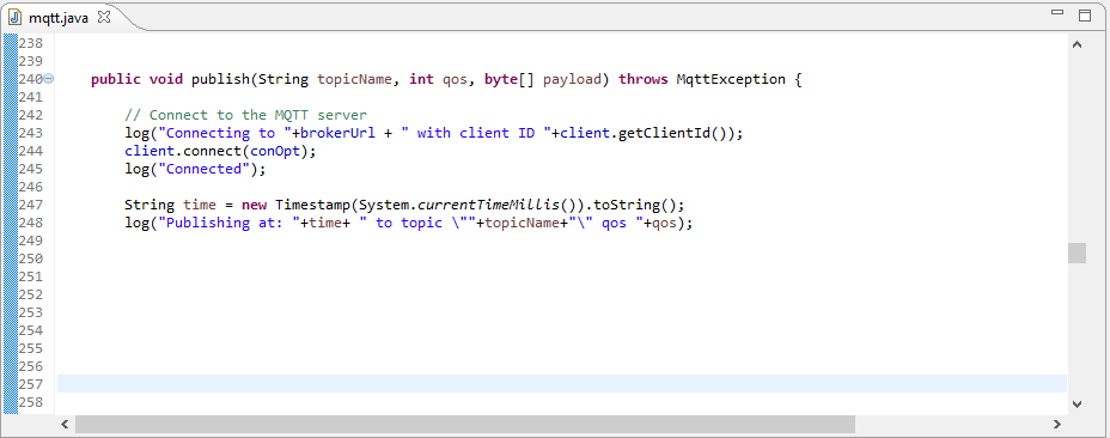
\includegraphics[width=\columnwidth]{figs/API-example} \\
	\scriptsize{a) Initial version} \\
	\vspace{.2cm}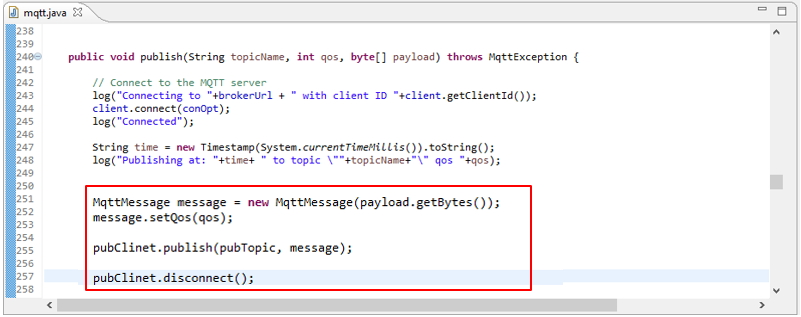
\includegraphics[width=\columnwidth]{figs/API-example-final} \\
	\scriptsize{b) Final version}\\
	\vspace{-.2cm}
	\caption{Use case study}
	\label{fig:codeExample}
\end{figure}

Fig.~\ref{fig:codeExample}.a depicts the situation where the development 
is at an early stage and the developer already used some methods of the chosen 
API to develop the required functionality. However, she is not sure how to 
proceed from this point. In such cases, different sources of information 
may be consulted, such as StackOverflow, video tutorials, API 
documentation, \etc. In this paper, we propose an approach aiming at providing 
developers with recommendations consisting of a list of API method 
calls that should be used next, and with usage patterns that can be used as a 
reference for completing the development of the method being defined (\eg code 
snippets that could support developers to complete the method definition with 
the framed code in Fig. \ref{fig:codeExample}.b).

	
	\section{Valuable features of a code search engine}
	\label{sec:Features}
	Considering all these information, we can list several features that should be taken into consideration and implemented during the development of a recommendation system based on retrieving source code. The key features are: 
\begin{itemize}
\item The query mechanism;
\item  The similarity criteria;
\item  How it indexes the data (if present);
\item The post-ranking process (if present);
\item The source of the recommended snippets (S0,Github);
\item The tool interoperability support  (plugin,Web client);
\item The supported languages;
\item Tool availability;
\item Validation framework of results

\end{itemize}
Of course, this list is only a small part of possible features but we have focused on this subset to perform a more complete and qualitative investigation on them. 	

	
	\section{Overview of existing approaches}
	\label{sec:RelatedWorks}
	At this point, we show an overview on the existing approaches by pointing out the technique and the main features in order to do the comparison with our approach. 

\subsection{Prompter}
We look at \cite{DBLP:journals/ese/PonzanelliBPOL16} in which the authors propose Prompter, an automatic tool to search and retrieve recommendations coming from SO. The key idea is to perform a web crawling activity in Google considering the developer's context. Given this context, composed by the source code, Prompter builds the query using the Query Generator Service (QGS) component. 
 To build the query, the authors use a naive approach, presented by Ponzanelli et al., that splits the identifiers and removes the stop word, ranks the terms according to their frequency and shows the top rank element. Moreover, they consider also the entropy of each term, according to Shannon's interpretation. Thus, Prompter uses the text quality index (TDI) to assess the goodness of the query, by considering the features described above. Once the proper component builds the query,  the QGS component sends it, with the context, to the Search Service that acts as an interface among the tool, the web engines (ie Google, Bing) and StackOverflow API that performs the crawling of the discussion. Finally, the authors use a ranking model to sort the results according to different metrics. We will see them in details as they represent a baseline to evaluate our approach. 
Concerning the final evaluation of the produced recommendations by Prompter, the authors made two studies to assess the quality of the tool: one relies on a survey in which the authors ask 55 people (with different skills and job experiences) to evaluate the Prompter's results in term of accuracy. In particular, the questions want to discover how much the developers use StackOverflow as support during the development (as well as Java API documentation or similar) and if the Prompter's suggestions are related (or not) to the context. 
The second study involves instead several programming tasks that the developer have to implement. Going in deep, the authors propose two kinds of task: a maintenance task (MT), that requires only little changes in the original code, and a development task (DT) in which the developer must implement multiple functionalities from scratch. The results claim that Prompter works well and, in particular, the developers indicate as valuable features the accuracy of suggestion and the user interface. On the other hand, the main limitations are the interface that doesn't allow to choose key terms during the search activity and the missing integration of a  search field, that forces the developer to exit from IDE and surf on Web. To validate all these results, the authors use R studio to apply statistical methods and functions. 


\subsection{FaCoY – A Code-to-Code Search Engine}
In this work, the authors propose a tool, Facoy,  to search similarity in snippets of code. Facoy uses Lucene to build and perform a query (and alternate versions of it) on SO dump. The aim is to find similar posts on SO considering the semantic and not only the syntactic structure of the snippet of code.  To do this,  the authors use Lucene to set indexes that represent the relationship between the code and the semantic. In particular, Facoy uses the snippet index to associate the answer document IDs with the code in the SO posts, by creating pairs in form of token\_type: actual\_token with Lucene. To generate all possible terms from the code, the authors parse the AST of the code, by wrapping the incomplete code in a dummy class if needed. The second index, called question index, maps the information between the question and the source code in the SO posts. Facoy uses this index to perform semantic analysis and try to find alternate queries that should cover more cases. Finally, Facoy uses the code index to search the similarity between the user's code and the code in the SO posts.  The tool builds the AST of the code (building dummy classes if needed), similarly with respect to the first index. Once the authors define these indexes, Facoy retrieves the results and, by using Lucene functions, it ranks the results. In particular, the tool exploits the Lucene function for textual similarities like Boolean Model and Vector Space model for scoring, plus TF-IDF for rank the result and to compute the Cosine similarity between the developer's code and indexed snippets. To evaluate the obtained results and assess the quality of the proposed tool, the authors set four different research questions about the precision and accuracy of Facoy against the other code search engines. As dataset, they consider 10.449 Github projects and the SO dump from 2008 to 2016. They focus on Java and Android code and index over 1.800.000 SO posts. From the evaluation, Facoy outperforms Krugle and Searchcode, the two code search engine considered in the comparison. 

\subsection{CodEX: Source Code Plagiarism Detection Based on Abstract Syntax Trees}
In this paper, the authors propose a tool to detect plagiarism in the source code. Codex, the proposed tool, analyzes the AST of the code and perform a similarity analysis based on fingerprints. In facts, it summarizes the AST of the code and then generates the respective fingerprint to represent relevant information of the tree. In particular, Codex gives a specific weight to each fingerprint, although it performs a relatively fine-grained analysis that consists in giving a lower score to so-called tiny terms (i.e. parameters or constant) that have less impact than bigger nodes in the tree. Moreover, the authors analyze also the occurrence of sibling functions and, finally, compare the fingerprints of the subtrees in a top-down manner. Considering these weights, Codex performs the search considering two levels of similarity: the local one, that compare the pair context-single snippet, and the global one, in which it compares the fingerprint of the developer's code with the whole corpus. To make these comparisons, the tool walks the ASTs and prunes unnecessary nodes, according to a given threshold. To assess the quality of Codex, the authors select 10 test cases with plagiarised code, 5 written in Python and 5 in Java. In particular, they consider different kinds of plagiarism, like code modification, comments insertion, block combination. The results show that Codex is able to recognize the duplicated code in almost test cases, with accuracy near to 90\%.

\subsection{CodeHow: Effective Code Search based on API Understanding and Extended Boolean Model}
In this work, the authors propose a code search engine, called CodeHow, that perform the code analysis by using two key concepts: the API documentation and the Extended Boolean model. Focusing on the whole process, CodeHow parsers the API online documentation by analyzing the user query. As the first step, the tool retrieves and parser the information coming from the documentation using the classical text preprocessing techniques (text normalization, stop words removal and stemming). In this way, CodeHow is able to find similarities between the user’s query and the API related to it. To identify the relevant APIs among all retrieved ones, the authors propose a different information retrieval technique, called the Extended Boolean Model (EBM). From the literature, we know that there are two main techniques to asses the similarity of two elements: the Boolean model, that assigns 0,1 as weights to elements, and the Vector Space Model (VSM), that summarizes documents using vectors and calculate usually the Cosine similarity on them. The EBM is a trade-off between the two previous techniques because it assigns weights that belongs to an interval (between 0 and 1) and then normalizes the metric using the p-value (in this paper, the authors set it to 3).
Coming back to the proposed approach, they use Elastic Seach to index the results, the classical VSM function already built-in in the Apache Lucene library and, finally, the Extend Boolean Model to build the query that achieves more results. In particular, they analyze a single term before assigning it a weight: if the term t is an API, CodeHow assigns to it the API score calculated by Lucene VSM; if the term is not an API, the tool uses the TF-IDF index to set the score. In order to evaluate the obtained results, the authors use a dataset composed of 26.000 C\# projects. Considering this dataset, they perform first an internal experiment, by performing 34 real queries coming from the literature and checking by hand the top 20 results for each query. Then, they perform a user evaluation involving 20 Microsoft developers who are called to implement three different tasks: the first one regards the sending emails, the second concerns the conversion from text to XML and the last the image format conversion. The authors compare their approach with Ohloh, another code search engine, and, from this comparison, CodeHow performs the analysis better than the opponent. Moreover, they evaluate the results with MRR and precision metrics already seen in other works.  


\subsection{Sourcerer: mining and searching internet-scale software repositories}
In this work, the authors propose Sourcerer, a tool that performs code search in the large-scale repositories. The first component involved in the processing is the crawler, that downloads automatically the repositories. Then, the tool analyzes the code involving three entities: the parser, that maps each repository to the entity and possible relationships, modeled by a relational database; Lucene, that indexes the entities using keywords included in the code. Beside this keyword-based technique, Sourcerer uses also the fingerprints, that summarize the snippets in vectors and give information about the syntactical information of the code. The tool uses them as support for structural search.  Finally, the third component is the ranker, based on the graph-based representation of the code to filter and retrieve top rank results, going beyond the text-based similarity. Additionally, it uses also fingerprints and keywords analysis, taking care of the best common practices in the computer science community (i.e name convention, analyzing the test classes, evaluating the complexity by LOC). Once Sourcerer made this kind of analysis and classification on the source code,  it maps also the authors of each snippet using a matrix with author-document entries. This kind of process gives further information about the developers who write the code: in particular, Sourcerer can categorize the authors with best skills according to their contributions. To evaluate the overall approach, the authors set up a user study on a dataset composed of over 4000 Java projects. They select 25 queries and do a manual evaluation  on the results, involving also three expert developers, considering four key aspects: the original content of the query and the topic of the search, the quality of the results in term of coverage, the reputation of the project and, finally, the possible reuse as a software component. Besides the human evaluation, they also use classical recall and precision metrics to assess the quality of the results from the statistical point of view. The results show that Sourcerer achieves high precision and accuracy considering the queries previously selected. 

\subsection{Retrieving Software Objects in an Example-Based Programming Environment}
In this work, the author proposes a tool, called CodeFinder, that performs recommendations using the example-based programming technique. As claimed in the paper, the most difficult part is to build the query and understand what the developer really needs. A system that relies only on a keyword-based system doesn't provide good enough results, because it excludes results that should be interesting for the user's purpose. Another problem strongly related to the example-based technique is that the suggested code doesn't fit exactly on the user's needs. To solve these issues, CodeFinder implements a hybrid approach that mixes the keyword-based style with information retrieval techniques, like the retrieval by reformulation that considers a subset of a concept instead try to match the exact one. To do this, the tool builds a network, that represents the conceptual model of the user, in which the keywords are induced by the query that the user is writing, using also the thesaurus to find synonyms that are more closer with respect to the query.  In the network, the keywords are the nodes and the relationship between them represent the level of likelihood. Once the user performs the first time the query, the CodeFinder interface retrieves other related keywords, the matching items and some code example of them. At this point, the interface allows adding new keywords in order to improve the query, exploiting the retrieval by reformulation technique. The key idea of this work is to guess the overall intentions of the developer when she writes some code, instead to reasoning only on the code or the query. Unfortunately, the validation of the tool is not available, as claimed by the author in the paper.

\subsection{Strathcona Example Recommendation Tool}
In this work, the authors propose Strathcona, a recommendation tool based on API. In particular, the tool analyzes the developer’s context from the structural point of view and suggests a possible implementation related to the task that she is developing. More in details, Strathcona uses six heuristics based on inheritance hierarchy, field types method calls and object usage in order to build the query. As the main similarity method, they use the structural context, based on the type of the classes and  type of their parents and fields, the signature of the methods while it doesn’t consider the name of fields, parameters and 
This query is performed on a repository, called the example repository, that contains all possible usage of the APIs and it is built automatically from the context. Strathcona retrieves the code examples related to the query that the developer can navigate both graphically and in a textual way. At this point, she can select the code examples that are more related to its task or can query again after she has written more code, to have more specific examples. The overall approach is informally validated by the University of Calgary. The main issue is that a typical user doesn’t know what is the starting point when she is implementing a completely new feature. The other issue is the quality of the example repository, that maybe not cover all possible cases. 





	
	\section{Proposed approach}
	\label{sec:ProposedApproach}
	\input{src/ProposedApproach}
	
	
	\section{Conclusion}
	\label{sec:Conclusion}
	\input{src/Conclusion}
	
	
	
	

	
	%\input{samplebody-conf}
	
	\balance
	\bibliographystyle{IEEEtranS}
	\bibliography{IEEEabrv,SurveyCodeSearchers}
	
\end{document}
